\documentclass{beamer}

\author[Dynamo Team]{
  Daniel Abercrombie \\
  Maxim Goncharov \\
  Yutaro Iiyama \\
  Benedikt Maier
}

\title{\bf \sffamily Dynamo -- Consistency Check}
\date{\today}

\usecolortheme{dove}

\usepackage[absolute,overlay]{textpos}
\usefonttheme{serif}
\usepackage{hyperref}
\usepackage[english]{babel}
\setbeamerfont{frametitle}{size=\Large,series=\bf\sffamily}
\setbeamertemplate{frametitle}[default][center]
\usepackage{siunitx}
\usepackage{tabularx}
\usepackage{makecell}

\setbeamertemplate{navigation symbols}{}
\usepackage{graphicx}
\usepackage{color}
\setbeamertemplate{footline}[text line]{\parbox{1.083\linewidth}{\footnotesize \hfill \insertshortauthor \hfill \insertpagenumber /\inserttotalframenumber}}
\setbeamertemplate{headline}[text line]{\parbox{1.083\linewidth}{\footnotesize \hspace{-0.083\linewidth} \textcolor{blue}{\sffamily \insertsection \hfill \insertsubsection}}}

\IfFileExists{/Users/dabercro/GradSchool/Presentations/MIT-logo.pdf}
             {\logo{\includegraphics[height=0.5cm]{/Users/dabercro/GradSchool/Presentations/MIT-logo.pdf}}}
             {\logo{\includegraphics[height=0.5cm]{/home/dabercro/MIT-logo.pdf}}}

\usepackage{changepage}

\graphicspath{{figs/}}

\newcommand{\link}[2]{\href{#2}{\textcolor{blue}{\underline{#1}}}}
\newcommand{\clink}[2]{\link{#1}{http://t3serv001.mit.edu/~dabercro/redir/?k=#2}}}

\newcommand{\twofigs}[4]{
  \begin{columns}
    \begin{column}{0.5\linewidth}
      \centering
      \textcolor{blue}{#1} \\
      \includegraphics[width=\linewidth]{#2}
    \end{column}
    \begin{column}{0.5\linewidth}
      \centering
      \textcolor{blue}{#3} \\
      \includegraphics[width=\linewidth]{#4}
    \end{column}
  \end{columns}
}

\begin{document}

\begin{frame}[nonumbering]
  \titlepage
\end{frame}

\begin{frame}
  \frametitle{We want to know what files are actually at each site}

  We compare what is physically at a site with what is
  expected to be there according to an inventory database.

  \begin{itemize}
  \item Sites may be missing files
    \begin{itemize}
    \item Can cause transfers to fail if source is invalid
    \item Sites are chosen incorrectly for production jobs
      that assume a local file
    \item Last disk copy might actually not be present,
      causing a delay when requested by a user
    \end{itemize}
  \item Some files may not be accounted for in our inventory
    \begin{itemize}
    \item Will not be used (besides accidentially through AAA)
    \item Wasting disk space
    \end{itemize}
  \end{itemize}

\end{frame}

\begin{frame}
  \frametitle{There is room for improving the old method}

  \begin{itemize}
  \item T0/T1 sites are checked twice a year
    \begin{itemize}
    \item Contact site admins
    \item Get site content
    \item Compare physical content with inventory
    \item Give admins lists of orphans and locally invalidate missing
    \end{itemize}
  \item T2 checked when problem suspected, on request
    \begin{itemize}
    \item May end in, \emph{e.g.}, local invalidation by hand
    \end{itemize}
  \end{itemize}

  Both of these processes are time-intensive, and manual.

  We should be able to delegate most of these tasks to a machine.

\end{frame}

\begin{frame}
  \frametitle{A simple automated procedure works}

  Over the past month,
  we have been automatically listing and correcting sites.

  \begin{itemize}
  \item Listing US T2s daily via XRootD calls
  \item Comparing results to Dynamo inventory and PhEDEx
  \item Missing and orphan files entered into registry
  \item Files handled in three ways:
    \begin{enumerate}
    \item Orphans are directly deleted
    \item Missing files on disk transfered with FTS
    \item Missing files only on tape locally invalidated
    \end{enumerate}
  \end{itemize}

  US T2 sites worked after communicating with admins
  to get permissions and to update their XRootD plugins.

\end{frame}

\begin{frame}
  \frametitle{At the end of August we were only listing a few sites}

  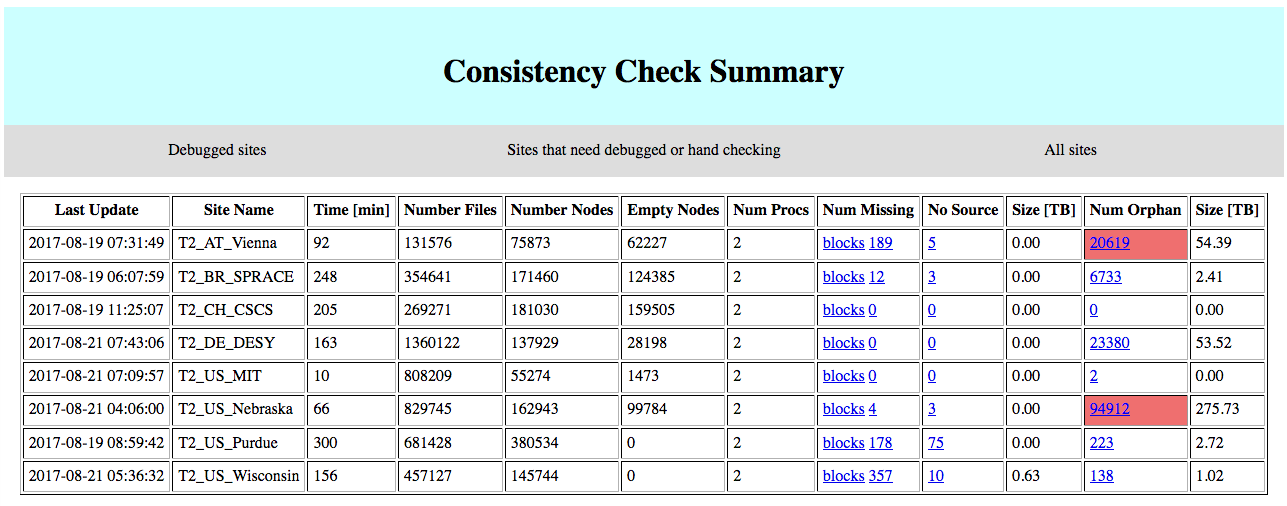
\includegraphics[width=\linewidth]{first_screenshot.png}

  Wanted to clean orphans from Nebraska.

\end{frame}

\begin{frame}
  \frametitle{Now listing US and some European T2s}

  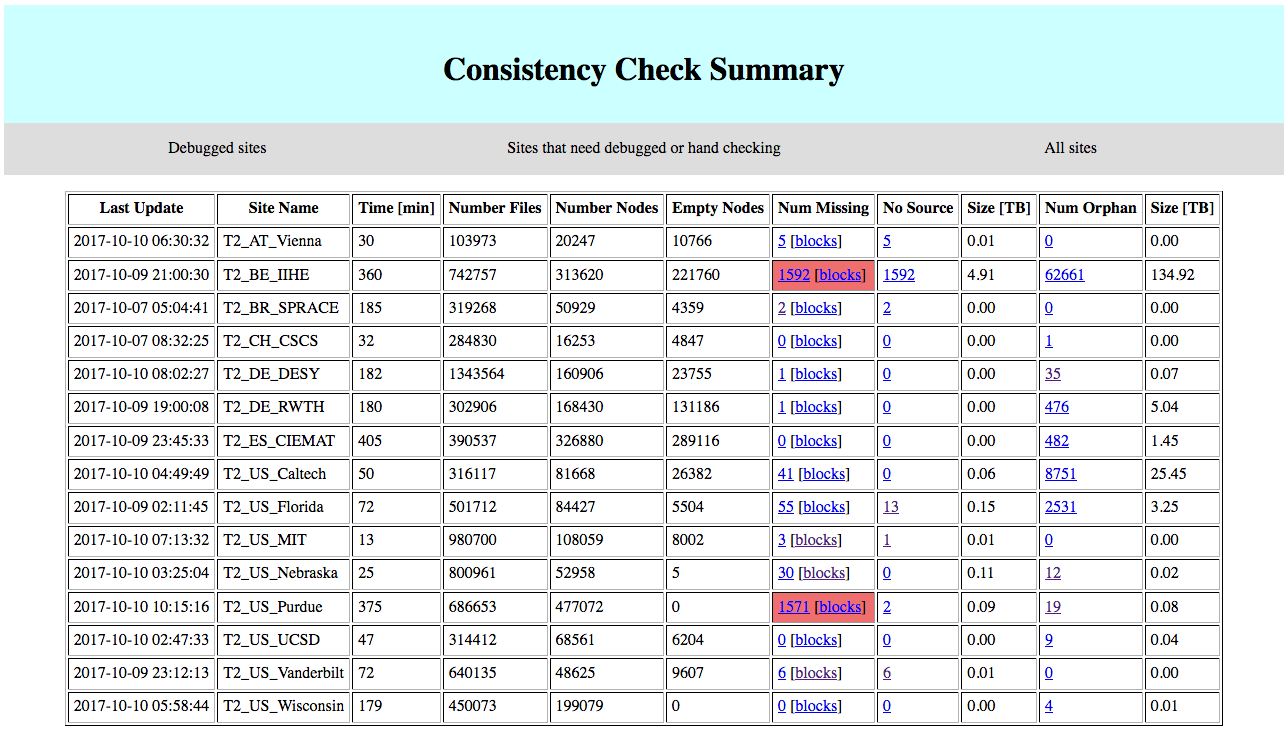
\includegraphics[width=\linewidth]{new_screenshot.png}

  \begin{itemize}
  \item Sites from the previous slide are generally more consistent
  \item Florida is recovering from storage system migration
  \end{itemize}

\end{frame}

\begin{frame}
  \frametitle{Consistency improvements made in past month}

  \centering
  \begin{tabular}{l | r | r}
    \hline
    Site & \multicolumn{1}{l|}{Recovered [TB]} & \multicolumn{1}{l}{Removed [TB]} \\
    & \multicolumn{1}{l|}{(was missing)} & \multicolumn{1}{l}{(was orphan)} \\
    \hline
    T2\_AT\_Vienna & 0.1 & 54 \\
    T2\_DE\_DESY & 0 & 100 \\
    T2\_US\_Caltech & 0 & 120 \\
    \hline
    T2\_US\_Florida & 300 (not all us) & 2 \\
    T2\_US\_Nebraska & 10 & 275 \\
%    T2\_US\_MIT &  \\ I literally don't remember
    T2\_US\_Purdue & 0.5 & 5 \\
    \hline
    T2\_US\_UCSD & 16 & 75 \\
    T2\_US\_Vanderbilt & 0 & 157 \\
    T2\_US\_Wisconsin & 0 & 2 \\
    \hline
  \end{tabular}

% MAKE COLUMN FOR EMPTY DIRECTORIES

  \vspace{8pt}
  \begin{itemize}
  \item T2\_US\_MIT was fixed during development, so we don't have full logs,
    but it had ~10s of TB of inconsistencies all recovered now
  \item Hundreds of thousands of empty directories have also been removed
    \textcolor{red}{Note to me: add column}
  \end{itemize}

\end{frame}

\begin{frame}
  \frametitle{Conclusions}

  \begin{itemize}
  \item In the past month, we have recovered around half a petabyte of disk space
    with minimal site admin or operator manual activity
  \item Recovering missing files is also progressing smoothly,
    using Florida's special case to stress test both FTS and invalidation tools
  \item After initial recoveries, quantity of requests will decrease
  \item A few European sites are also benefitting already
  \end{itemize}

\end{frame}

\end{document}
